\section{Тележка и меандр} 
\subsection{Математическая модель}
Рассмотрим математическую модель тележки, взяв за выходной сигнал линейную 
координату тележки $x$ и за входной сигнал силу $u$ на тележку. 
Тогда модель тележки в форме вход-состояние-выход имеет вид
\begin{equation}
    \begin{cases}
        \begin{bmatrix}
            \dot{x} \\ 
            \ddot{x} \\
        \end{bmatrix} = 
        \begin{bmatrix}
            0 & 1 \\ 
            0 & 0 \\
        \end{bmatrix} \times \begin{bmatrix}
            x \\ 
            \dot{x} \\
        \end{bmatrix} + \begin{bmatrix}
            0 \\ 
            1 \\
        \end{bmatrix} \times u  \\
        y = \begin{bmatrix}
            1 & 0 \\
        \end{bmatrix} \times \begin{bmatrix}
            x \\ 
            \dot{x} \\
        \end{bmatrix}
    \end{cases}
\end{equation}
или же, в более удобном для работы виде
\begin{equation}
    \begin{cases}
        \hat{x} = Ax + Bu \\ 
        y = Cx
    \end{cases}
\end{equation}
где     
\begin{equation}
    \begin{array}{ccc}
        A = \begin{bmatrix}
            0 & 1 \\ 
            0 & 0 \\
        \end{bmatrix}, & 
        B = \begin{bmatrix}
            0 \\ 
            1 \\
        \end{bmatrix}, ? 
        C = \begin{bmatrix}
            1 & 0 \\
        \end{bmatrix}
    \end{array}
\end{equation}

\subsection{Входное воздействие}
В качестве задающего воздействия рассмотрим меандр с периодом $T = 3$. 
Входное воздействие имеет вид
\begin{equation}
    u(t) = 
    \begin{cases}
        1, & t \in [1, 2) \\
        2, & t \in [2, 4)
    \end{cases}
    \label{eq:func_1}
\end{equation}

Разложим его в ряд Фурье с ограниченным числом гармоник для нахождения 
приближенного сигнала входного воздействия, которой можно будет использовать для 
синтеза регулятора.

\begin{equation}
    F_N(t) = \frac{a_0}{2} + \sum\limits_{n=1}^{N} \left( a_n \cos(\omega_n t) + b_n \sin(\omega_n t) \right)
    \label{eq:fourier}
\end{equation}
\begin{equation}
    a_n = \frac{2}{T} \int\limits_{h}^{h + T} f(t) \cos(\omega_n t) dt ~~~~ b_n = \frac{2}{T} \int\limits_{h}^{h + T} f(t) \sin(\omega_n t) dt 
    \label{eq:fourier_coefficients}
\end{equation}
где $\omega_n = 2\pi n / T$, $h$ -- начало промежутка, на котором проводится разложение, $T$ -- период функции.

\begin{equation}
    a_n = \frac{2}{3} \int\limits_{1}^{4} f_1(t) \cos\left( \frac{2\pi n}{3} t\right) dt = \frac{2}{3} \left( \int\limits_{1}^{2} \cos\left( \frac{2\pi n}{3} t\right) dt + \int\limits_{2}^{4} 2 \cos\left( \frac{2\pi n}{3} t\right) dt \right) 
\end{equation}
\begin{equation}
    b_n = \frac{2}{3} \int\limits_{1}^{4} f_1(t) \sin\left( \frac{2\pi n}{3} t\right) dt = \frac{2}{3} \left( \int\limits_{1}^{2} \sin\left( \frac{2\pi n}{3} t\right) dt + \int\limits_{2}^{4} 2 \sin\left( \frac{2\pi n}{3} t\right) dt \right) 
\end{equation}

Найдем первые 8 элементов ряда:
\begin{table}[ht!]
    \centering
    \begin{tabular}{|c|c|c|c|}
        \hline
        $n$ & $a_n$ & $b_n$ \\
        \hline
        0 & 3.33335 & 0.0 \\
        1 & 0.55123 & 0.0 \\
        2 & -0.2757 & 0.0 \\
        3 & 0.00020 & 0.0 \\
        4 & 0.13773 & 0.0 \\
        5 & -0.11037 & 0.0 \\
        6 & 0.00020 & 0.0 \\
        7 & 0.07866 & 0.0 \\
        8 & -0.06902 & 0.0 \\
        \hline
    \end{tabular}
    \caption{Коэффициенты Фурье для функции $u(t)$}
\end{table}

Функция $u(t)$ и ее частичный ряд Фурье с 8 гармониками изображены на рисунке \ref{fig:fourier}.
\begin{figure}[ht!]
    \centering
    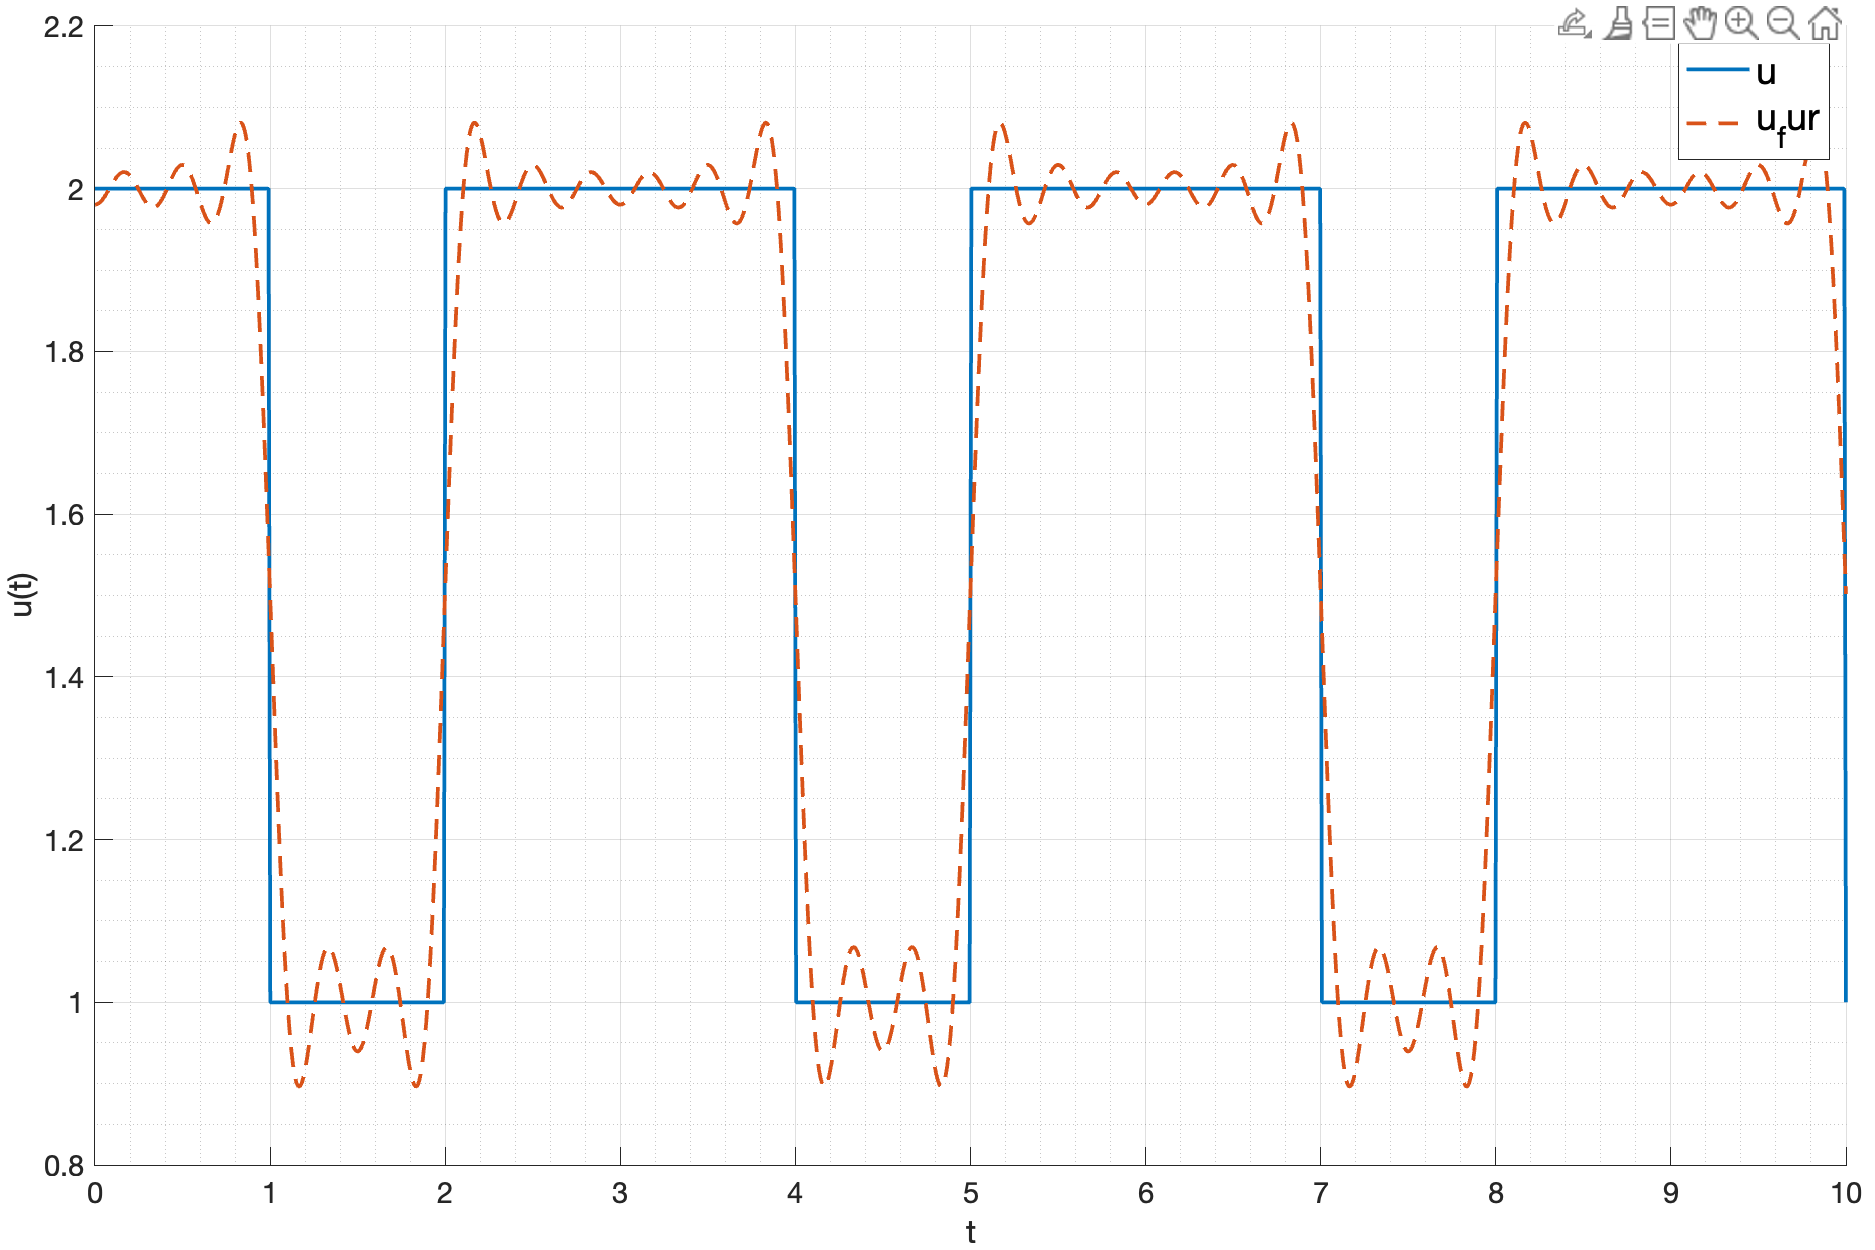
\includegraphics[width=\textwidth]{media/plots/u_fourier.png}
    \caption{Функция $u(t)$ и ее частичный ряд Фурье с 8 гармониками}
    \label{fig:fourier}
\end{figure}

При этом аналитически сигнал будет выглядеть следующим образом:
\begin{equation}
    g(t) = 
\end{equation}

\subsection{Формирование генератора}
Для того, чтобы составить генератор, дающий на выходе функцию, соответствующую частичному ряду 
Фурье, зададим матрицу $\Gamma$ как блочную Жорданову матрицу, каждой блок которой будет отвечать 
одной гармонике. 
